\chapter{Principle Component Analysis}

\section{Theory}
\emph{Principle Component Analysis} is a process by which a multivariate data set, containing observations in multiple features, can be reduced to a data set with a lower dimensionality, aiding in computational complexity and visualization\footnote{It's quite difficult to plot data in 17-dimensional space, for example, but quite easy to plot data in 2-dimensional space.}. PCA works by attempting to identify various new features which maximize the variance of the original data, and from which we could most easily reconstruct the original characteristics of our observations.

These new features (the \emph{principle components} in PCA) act as a new set of axes along which we can plot and analyze our data. These components are identified using eigenvalue/eigenvector decomposision.\footnote{Recall that an \emph{eigenvector} is a vector which is not rotated under a linear transformation, it is only scaled. The scale factor, denoted by $\lambda$, is called the \emph{eigenvalue} of that vector.} Specifically, we preform decompoisition on the covariance matrix $\Sigma$ of our data. Consider an imaginary data set which has $m$ observations (perhaps of different celestial objects) in $n$ different features (color, redshift, right ascension, declination, etc.). The covariance matrix of this data set will be an $n \times n$ square matrix, where the $(i,j)$ entry represents the covariance of the $i$\textsuperscript{th} and $j$\textsuperscript{th} features in our data. Importantly, it is useful to note that $\Sigma$ is a \emph{square symmetric} matrix, since the covariance of the $i$\textsuperscript{th} and $j$\textsuperscript{th} features equals the covariance of the $j$\textsuperscript{th} and $i$\textsuperscript{th} features; mathematically,
\[ \operatorname{Cov}(X_i,X_j) = \operatorname{Cov}(X_j,X_i) \implies \Sigma_{ij} = \Sigma_{ji}. \]
Since $\Sigma$ is square symmetric, we know it is diagonalizable\footnote{This is a direct consequence of the \emph{spectral theorem}.} into a new matrix whose entries are the eigenvalues of the principle components of the data set. Each eigenvalue represents the variance of the data along that new axis.
\[ \Sigma \sim \begin{pmatrix}
\lambda_1 & 0 & 0 & \cdots \\
0 & \lambda_2 & 0 & \cdots \\
0 & 0 & \lambda_3 & \cdots \\
\vdots & \vdots & \vdots & \ddots
\end{pmatrix} \]
By selecting the $k$ largest eigenvalues, we can reduce our original data set from $n$-dimensional space into $k$-dimensional space. The smaller our value of $k$, the simpler our model becomes, but we pay a price of explaining less and less of the underlying variance in the data. Our goal will be to strike a happy medium between the two, reducing our data to a visualizable range but preserving enough of the variation that we don't loose too much information.

\section{Application to SDSS Data}
As noted in the introduction, one of the greatest things about data from the Sloan Digital Sky Survey is that it has observations in many different features. The quasar data used in this project has 23 distinct values for each observation. Among these, one is a designation within the SDSS catalogue, and eight are error values for other observations. These values are not measured quantities, and don't really serve to explain observational features we might wish to use to analyze our data, so we won't include these in our original data set when preforming PCA.
\begin{marginfigure}
	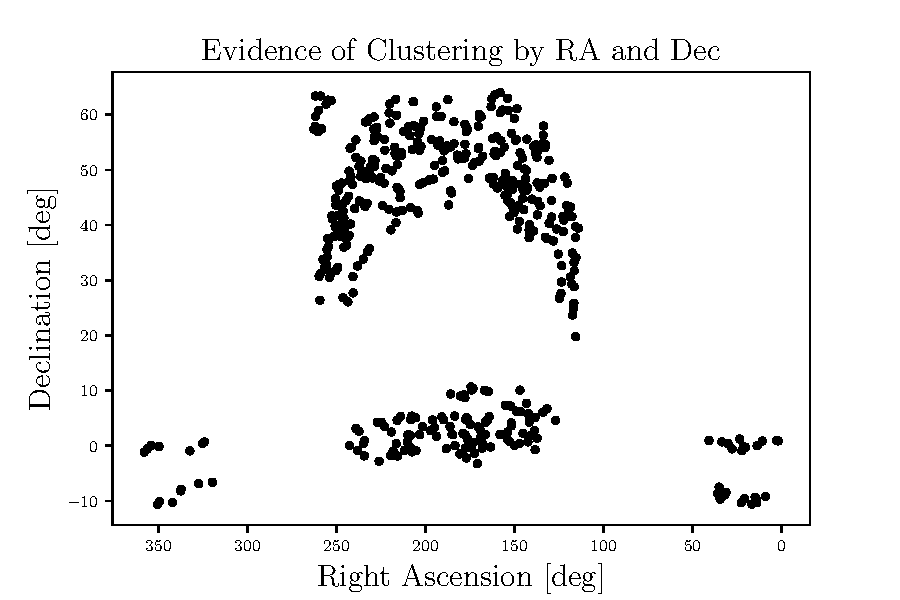
\includegraphics[width=2.3in]{ra-dec}
	\caption{Evidence of clustering in \texttt{RA} vs \texttt{Dec}. These clusters are apparent because the SDSS data only contains observations for certain regions of the sky, not because the data are demonstrative of quasar clusters in particular regions.}
	\label{fig:ra-dec}
\end{marginfigure}
\begin{marginfigure}
	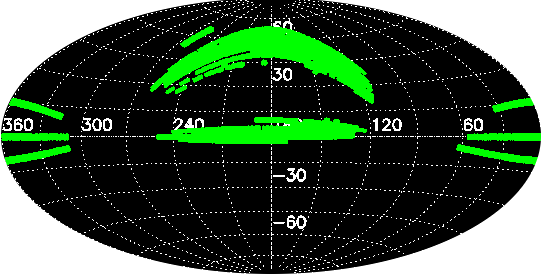
\includegraphics[width=2.3in]{dr3spectro_big}
	\caption{Map of spectral coverage from SDSS Data Release 3~[\cite{sdssWebsite}].}
	\label{fig:spec-cov}
\end{marginfigure}
Additionally, data in the \texttt{K\_mag}, \texttt{H\_mag}, and \texttt{J\_mag} features contain \texttt{NA} values when no value was observed for a particular quasar; if we included these three features in our analysis, PCA would find that the \texttt{NA} values would serve as an indicator for a group which doesn't exist, so these features are excluded from the analysis as well. Finally, we remove the Right Ascension and Declination values from the data, since the data form distinct observational clusters which arise from the limitations of the survey, and are not representative of actual clustering found in nature. Compare the \texttt{RA} vs \texttt{Dec} plot of quasar data in Figure~\ref{fig:ra-dec} to the map of spectral coverage from SDSS Data Release 3 in Figure~\ref{fig:spec-cov}. This leaves the data set with nine distinct features for analysis.

Observations of radio and X-ray brightness also contain some missing values; since these values come from compilations of different astronomical surveys (NRAO FIRST for radio data, ROAST All-Sky Survey for X-ray data), it only makes sense to include observations which have complete data in both categories. Thus, we must mask our original data to exclude partial observations, or else the \texttt{NA} values present will again serve as indicator variables for clusters which don't exist. Fully reducing our data set, we are left with $456$ observations in $9$ features.

We conduct Principle Component Analysis on the data using \texttt{scikit-learn}'s \texttt{PCA} tool. The first task is to find the optimum number of components to which we should reduce our data. Such a value is found by comparing the explained variance in the reduced data set by the number of components in that data set. In general, we expect that increasing the number of components will explain more of the variance in the data, but increasing the number of components too much will result in data that cannot be easily visualized.
% or worked with in a meaningfully more efficient way than working with the unreduced data would entail.

\begin{figure}
	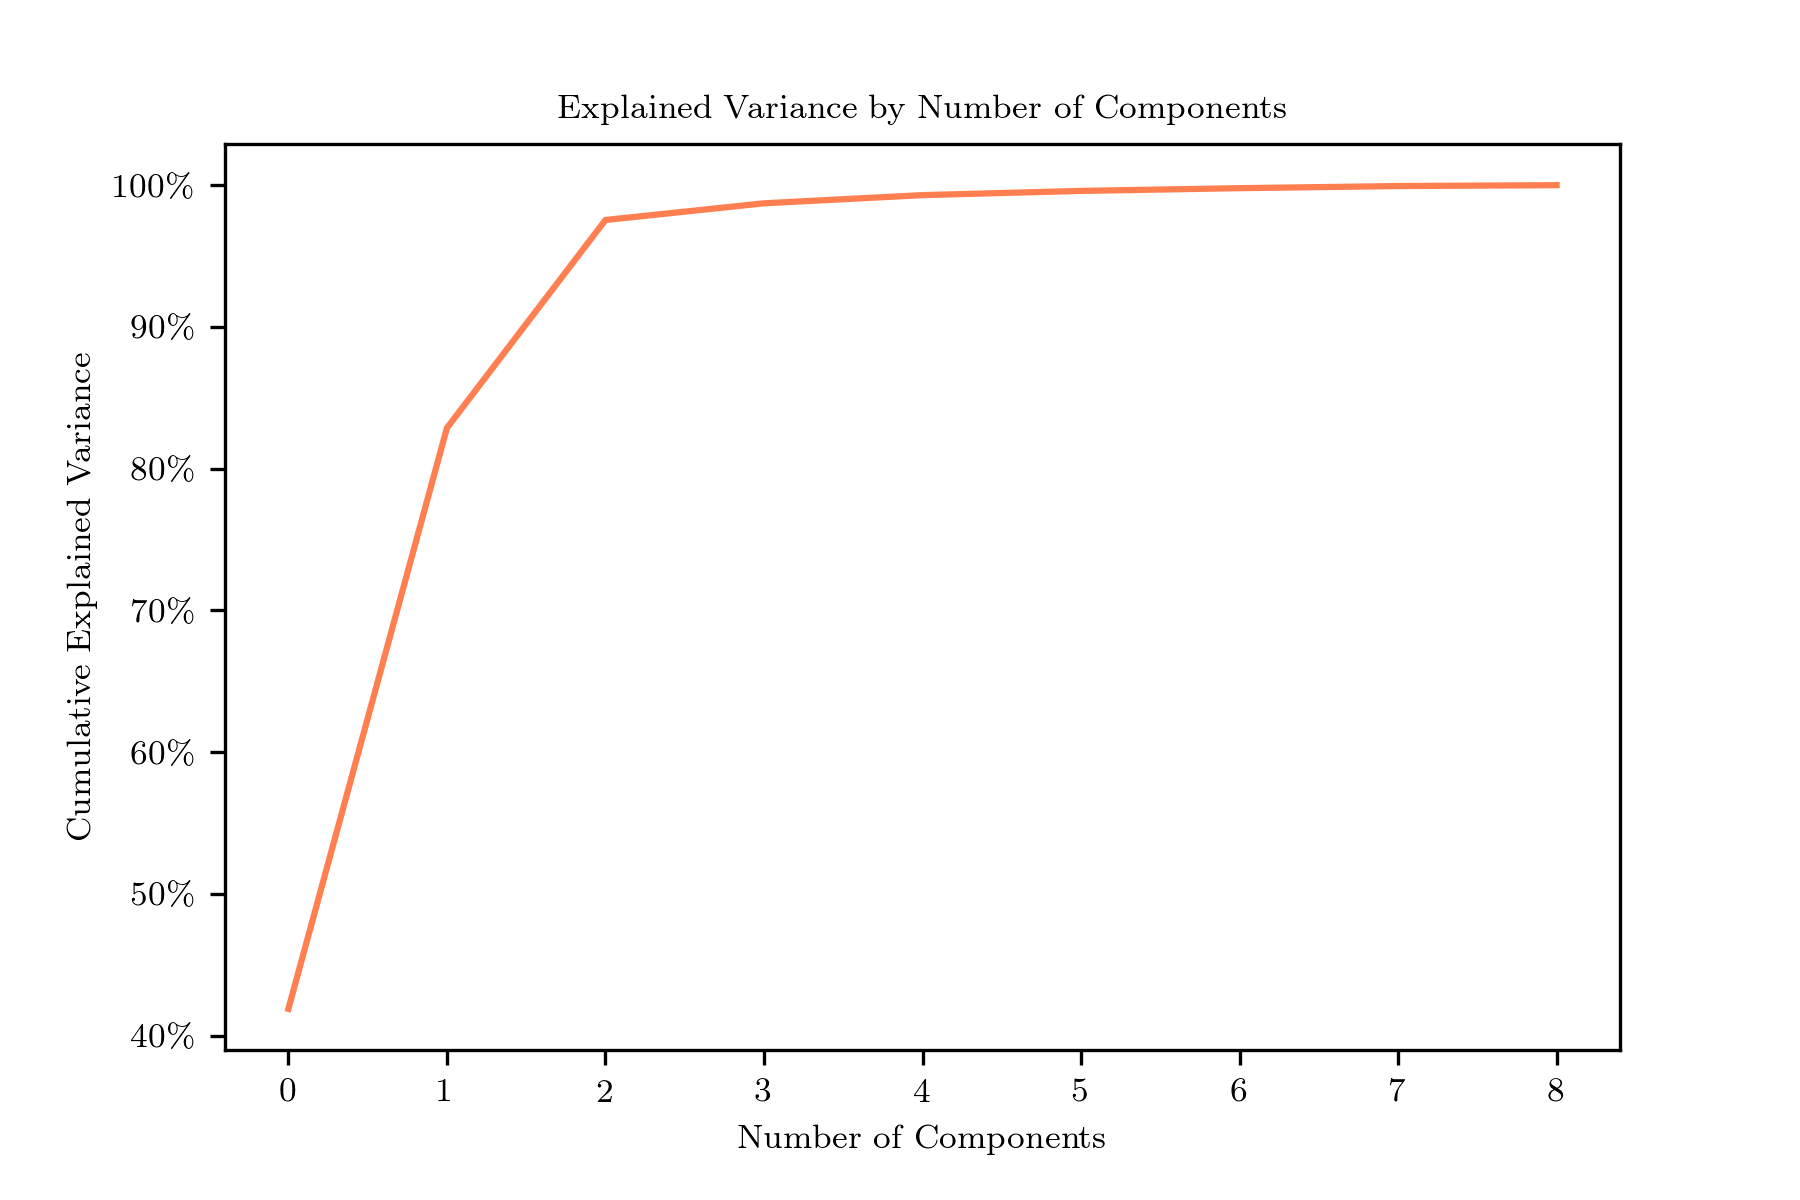
\includegraphics[width=\textwidth]{exp-var}
	\caption{As we increase the number of components in our reduced data set, the explained variance increases. Notice that after $n=2$, each additional component contributes minimally to the cumulative explained variance.}
	\label{fig:exp-var}
\end{figure}

As shown in Figure~\ref{fig:exp-var}, we find that the first two principle components explain over $97.5\%$ of the total variance in our data set, indicating that we can safely reduce the dimensonality of the quasar data to just two components. For ach additional component ($n = 3, \dots, 8$), we see diminishing returns to how much we can explain the variance in our data. Adding a third principle component gets us to $98.7\%$ of the total variance, and a fourth pushes us to over $99\%$ of the total variance, but we loose the ability to adequately visualize the data.

\begin{figure}
	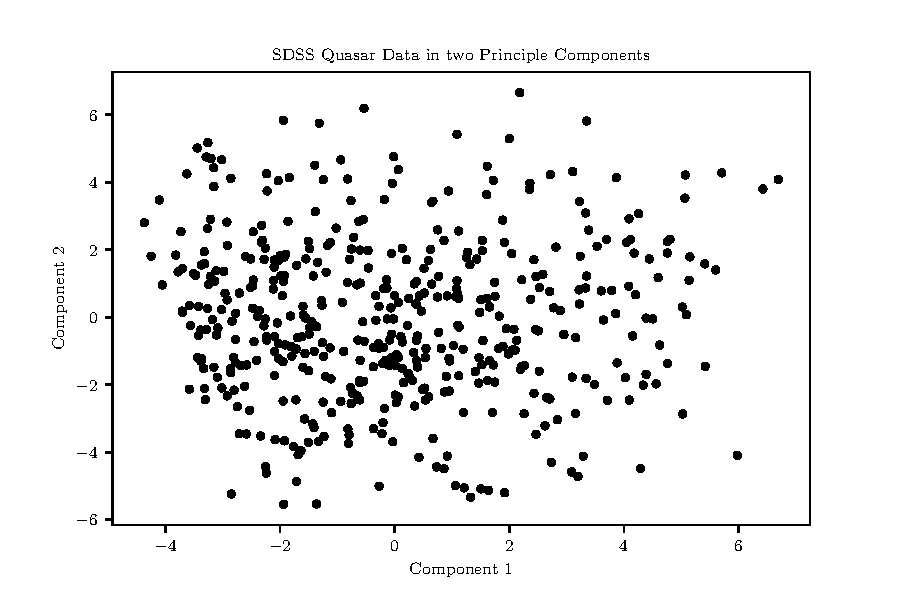
\includegraphics[width=\textwidth]{pca-reduced}
	\caption{Our original 456 observations in 9-dimensional data projected into a two-dimensional visualization.}
	\label{fig:pca-red}
\end{figure} 
While Figure~\ref{fig:pca-red} shows it is now much easier to graph our data, we do lose about $2.5\%$ of the total explained variance using this lower-dimensional model. We also lose the ability to physically understand exactly \emph{what} each axis represents. While before, we could have plotted the data in color-radio magnitude space, we now only have `Component 1' and `Component 2', which represent some linear combination of the original features.